\documentclass[11pt]{article}

\usepackage{fullpage}
\usepackage{amsmath, amssymb, bm, cite, epsfig, psfrag}
\usepackage{graphicx}
\usepackage{float}
\usepackage{amsthm}
\usepackage{amsfonts}
\usepackage{listings}
\usepackage{cite}
\usepackage{hyperref}
\usepackage{tikz}
\usepackage{enumerate}
\usepackage{mcode}
\usetikzlibrary{shapes,arrows}
%\usetikzlibrary{dsp,chains}

%\restylefloat{figure}
%\theoremstyle{plain}      \newtheorem{theorem}{Theorem}
%\theoremstyle{definition} \newtheorem{definition}{Definition}

\def\del{\partial}
\def\ds{\displaystyle}
\def\ts{\textstyle}
\def\beq{\begin{equation}}
\def\eeq{\end{equation}}
\def\beqa{\begin{eqnarray}}
\def\eeqa{\end{eqnarray}}
\def\beqan{\begin{eqnarray*}}
\def\eeqan{\end{eqnarray*}}
\def\nn{\nonumber}
\def\binomial{\mathop{\mathrm{binomial}}}
\def\half{{\ts\frac{1}{2}}}
\def\Half{{\frac{1}{2}}}
\def\N{{\mathbb{N}}}
\def\Z{{\mathbb{Z}}}
\def\Q{{\mathbb{Q}}}
\def\R{{\mathbb{R}}}
\def\C{{\mathbb{C}}}
\def\argmin{\mathop{\mathrm{arg\,min}}}
\def\argmax{\mathop{\mathrm{arg\,max}}}
%\def\span{\mathop{\mathrm{span}}}
\def\diag{\mathop{\mathrm{diag}}}
\def\x{\times}
\def\limn{\lim_{n \rightarrow \infty}}
\def\liminfn{\liminf_{n \rightarrow \infty}}
\def\limsupn{\limsup_{n \rightarrow \infty}}
\def\GV{Guo and Verd{\'u}}
\def\MID{\,|\,}
\def\MIDD{\,;\,}

\newtheorem{proposition}{Proposition}
\newtheorem{definition}{Definition}
\newtheorem{theorem}{Theorem}
\newtheorem{lemma}{Lemma}
\newtheorem{corollary}{Corollary}
\newtheorem{assumption}{Assumption}
\newtheorem{claim}{Claim}
\def\qed{\mbox{} \hfill $\Box$}
\setlength{\unitlength}{1mm}

\def\bhat{\widehat{b}}
\def\ehat{\widehat{e}}
\def\hhat{\widehat{h}}

\def\phat{\widehat{p}}
\def\qhat{\widehat{q}}
\def\rhat{\widehat{r}}
\def\shat{\widehat{s}}
\def\uhat{\widehat{u}}
\def\ubar{\overline{u}}
\def\vhat{\widehat{v}}
\def\xhat{\widehat{x}}
\def\xbar{\overline{x}}
\def\zhat{\widehat{z}}
\def\zbar{\overline{z}}
\def\la{\leftarrow}
\def\ra{\rightarrow}
\def\MSE{\mbox{\small \sffamily MSE}}
\def\SNR{\mbox{\small \sffamily SNR}}
\def\SINR{\mbox{\small \sffamily SINR}}
\def\arr{\rightarrow}
\def\Exp{\mathbb{E}}
\def\var{\mbox{var}}
\def\Tr{\mbox{Tr}}
\def\tm1{t\! - \! 1}
\def\tp1{t\! + \! 1}

\def\Xset{{\cal X}}

\newcommand{\one}{\mathbf{1}}
\newcommand{\abf}{\mathbf{a}}
\newcommand{\bbf}{\mathbf{b}}
\newcommand{\dbf}{\mathbf{d}}
\newcommand{\ebf}{\mathbf{e}}
\newcommand{\gbf}{\mathbf{g}}
\newcommand{\hbf}{\mathbf{h}}
\newcommand{\hbfhat}{\widehat{\mathbf{h}}}
\newcommand{\pbf}{\mathbf{p}}
\newcommand{\pbfhat}{\widehat{\mathbf{p}}}
\newcommand{\qbf}{\mathbf{q}}
\newcommand{\qbfhat}{\widehat{\mathbf{q}}}
\newcommand{\rbf}{\mathbf{r}}
\newcommand{\rbfhat}{\widehat{\mathbf{r}}}
\newcommand{\sbf}{\mathbf{s}}
\newcommand{\sbfhat}{\widehat{\mathbf{s}}}
\newcommand{\ubf}{\mathbf{u}}
\newcommand{\ubfhat}{\widehat{\mathbf{u}}}
\newcommand{\utildebf}{\tilde{\mathbf{u}}}
\newcommand{\vbf}{\mathbf{v}}
\newcommand{\vbfhat}{\widehat{\mathbf{v}}}
\newcommand{\wbf}{\mathbf{w}}
\newcommand{\wbfhat}{\widehat{\mathbf{w}}}
\newcommand{\xbf}{\mathbf{x}}
\newcommand{\xbfhat}{\widehat{\mathbf{x}}}
\newcommand{\xbfbar}{\overline{\mathbf{x}}}
\newcommand{\ybf}{\mathbf{y}}
\newcommand{\zbf}{\mathbf{z}}
\newcommand{\zbfbar}{\overline{\mathbf{z}}}
\newcommand{\zbfhat}{\widehat{\mathbf{z}}}
\newcommand{\Ahat}{\widehat{A}}
\newcommand{\Abf}{\mathbf{A}}
\newcommand{\Bbf}{\mathbf{B}}
\newcommand{\Cbf}{\mathbf{C}}
\newcommand{\Bbfhat}{\widehat{\mathbf{B}}}
\newcommand{\Dbf}{\mathbf{D}}
\newcommand{\Gbf}{\mathbf{G}}
\newcommand{\Fbar}{\overline{F}}
\def\Hhat{\widehat{H}}
\newcommand{\Hbf}{\mathbf{H}}
\newcommand{\Kbf}{\mathbf{K}}
\newcommand{\Pbf}{\mathbf{P}}
\newcommand{\Phat}{\widehat{P}}
\newcommand{\Qbf}{\mathbf{Q}}
\newcommand{\Rbf}{\mathbf{R}}
\newcommand{\Rhat}{\widehat{R}}
\newcommand{\Sbf}{\mathbf{S}}
\newcommand{\Ubf}{\mathbf{U}}
\newcommand{\Vbf}{\mathbf{V}}
\newcommand{\Wbf}{\mathbf{W}}
\newcommand{\Xhat}{\widehat{X}}
\newcommand{\Xbf}{\mathbf{X}}
\newcommand{\Ybf}{\mathbf{Y}}
\newcommand{\Zbf}{\mathbf{Z}}
\newcommand{\Zhat}{\widehat{Z}}
\newcommand{\Zbfhat}{\widehat{\mathbf{Z}}}
\def\alphabf{{\boldsymbol \alpha}}
\def\betabf{{\boldsymbol \beta}}
\def\betahat{\widehat{\beta}}
\def\mubf{{\boldsymbol \mu}}
\def\lambdabf{{\boldsymbol \lambda}}
\def\etabf{{\boldsymbol \eta}}
\def\xibf{{\boldsymbol \xi}}
\def\taubf{{\boldsymbol \tau}}
\def\sigmahat{{\widehat{\sigma}}}
\def\thetabf{{\bm{\theta}}}
\def\thetabfhat{{\widehat{\bm{\theta}}}}
\def\thetahat{{\widehat{\theta}}}
\def\mubar{\overline{\mu}}
\def\muavg{\mu}
\def\sigbf{\bm{\sigma}}
\def\etal{\emph{et al.}}
\def\Ggothic{\mathfrak{G}}
\def\Pset{{\mathcal P}}
\newcommand{\bigCond}[2]{\bigl({#1} \!\bigm\vert\! {#2} \bigr)}
\newcommand{\BigCond}[2]{\Bigl({#1} \!\Bigm\vert\! {#2} \Bigr)}


\begin{document}

\title{EE6333:  Homework 3\\
Bayesian Estimation}
\author{Prof.\ Sundeep Rangan}
\date{}

\maketitle


\begin{enumerate}

\item 
\begin{enumerate}[(a)]
\item The MAP estimate is
\[
    \xhat = \argmax_x p(x|y) = \argmax_x C(y)e^{-H(x,y)}
    = \argmin_x H(x,y),
\]
where we have used the fact that $C(y)$ does not depend on 
$x$.

\item Using the fact that the density must integrate to one,
\[
    1 = \int p(x|y)dx = C(y)\int e^{-H(x,y)}dx = C(y)Z_0.
\]
Hence, $C(y)=1/Z_0$.  Therefore,
\[
    \Exp(x|y) = \int xp(x|y)dx = \frac{1}{Z_0}
    \int xe^{-H(x,y)}dx = \frac{Z_1}{Z_0}.
\]
Similarly,
\[
    \Exp(x^2|y) = \int x^2p(x|y)dx = \frac{1}{Z_0}
    \int x^2e^{-H(x,y)}dx = \frac{Z_2}{Z_0},
\] 
and hence
\[
    \var(x|y) =\Exp(x^2|y) -\Exp^2(x|y) = 
    \frac{Z_2}{Z_0} - \frac{Z_162}{Z_0^2}.
\]

\item Given the joint density $p(x,y)$ the posterior is 
\[
    p(x|y) = \frac{p(x,y)}{p(y)} = \frac{C(y)}{p(y)}e^{-H(x,y)}
        = C'(y)e^{-H(x,y)},
\]
where $C'(y) = C(y)/p(y)$. Hence, posterior $p(x|y)$ is in the same
form as in part (a), only with a different function $C(y)$.

\end{enumerate}

\item \label{prob:softThresh}
\begin{enumerate}[(a)] 
\item Since this is an AWGN channel, the ML estimate is
\[
    \thetahat = \argmin_{\theta \geq 0} (x-\theta)^2.
\]
Since the minimization is to be performed over $\theta \geq 0$,
we have the solution
\[
    \thetahat =  \begin{cases}
        0  & \mbox{if } x \leq 0 \\
        x  & \mbox{if } x \geq 0.
        \end{cases}
\]
Equivalently, we can write $\theta = \max\{x,0\}$.

\item From Bayes' rule, the posterior density is
\beq \label{eq:pthx}
     p(\theta|x) = \frac{1}{p(x)}p(x|\theta)p(\theta) 
    = \frac{1}{p(x)\sqrt{2\pi}\sigma \lambda}
    \exp\left[ -\frac{(x-\theta)^2}{2\sigma^2} - \frac{\theta}{\lambda} \right].
\eeq
Hence, we can take
\[
    H(\theta,x) = \frac{(x-\theta)^2}{2\sigma^2} 
    + \frac{\theta}{\lambda},
    \quad C(x) = \frac{1}{p(x)\sqrt{2\pi}\sigma \lambda}.
\]

\item 
From the previous problem 
\[
    \thetahat  = \argmin_{\theta \geq 0} H(\theta,x). \label{eq:Hmin}
\]
When we have hard constraint of the form $\theta \geq 0$, we break
this minimization into two cases: Either $\theta > 0$
or $\theta=0$.  If $\theta > 0$, then the minimum is in an open
neighborhood of the feasible set, so 
$\partial H(\theta,x)/\partial \theta = 0$ which implies
\[
    \frac{\theta-x}{\sigma^2} + \frac{1}{\lambda} = 0 
    \Rightarrow \thetahat = x - \frac{\sigma^2}{\lambda}.
\]
In order that $\thetahat > 0$, we need that $x \geq \sigma^2/\lambda$.
If this condition is not satisfied, then there cannot be a minima
with $\thetahat > 0$.  Hence, we must have $\thetahat = 0$.
We conclude that the MAP estimate is
\[
    \thetahat = \begin{cases}
        0           & \mbox{if } x \leq t \\
        x-t  & \mbox{if } x \geq t,
        \end{cases} \quad t = \sigma^2/t.
\]

\item Define
\[
    \mu = x - \frac{\sigma^2}{\lambda},
\]
so that
\[
    \frac{(\theta-x)^2}{2\sigma^2} + \frac{\theta}{\lambda}
    = \frac{(\theta-\mu)^2}{2\sigma^2} + \frac{x^2 - t^2}{2\sigma^2}.
\]
Hence, from \eqref{eq:pthx}, for $\theta > 0$,
\[
    p(\theta|x) = \frac{1}{p(x)\sqrt{2\pi}\sigma \lambda}
    \exp\left[ \frac{x^2 - t^2}{2\sigma^2} \right]
    \exp\left[ -\frac{\theta-\mu}{2\sigma^2} \right]
    = C(x)\phi\left(\frac{(\theta-\mu)^2}{\sigma}\right),
\]
where $C(x)$ is a function that depends only on $x$ 
(and not $\theta$) and $\phi(u)$ is the pdf of the standard Gaussian
\beq \label{eq:pthxbnd}
    \phi(u) = \frac{1}{\sqrt{2\pi}}e^{-u^2/2}.
\eeq
Since \eqref{eq:pthxbnd} is restricted to $\theta > 0$, this
is identical the truncated normal distribution  
$\theta \sim {\mathcal N}(\mu,\sigma)$ restricted to $\theta in [a,b]$
where $a=0$ and $b=\infty$.  From the wikipedia page
the posterior mean is
\[
    \Exp(\theta|x) = \mu + \frac{\phi(u)\sigma}{Q(u)},
\]
where $u=-\mu/\sigma$.

\item We can compute the estimates with the following code:
\begin{lstlisting}
% Parameters
lam = 1;        % Exp(theta)
wvar = 0.1;     % noise variance
nx = 200;       % number of points
x = linspace(-2,3,nx)'; % points to test

% ML estimate
xml = max(0,x);

% MAP estimate
t = wvar/lam;
mu = x-t;
xmap = max(0, mu);

% Compute MMSE estimate
u = -mu/sqrt(wvar);
phiu = 1/sqrt(2*pi)*exp(-u.^2/2);
xmmse = mu + sqrt(wvar)*phiu./qfunc(u);

% Plot the results
plot(x,[xml xmap xmmse],'-','Linewidth',2);
grid on;
set(gca,'FontSize',16);
legend('ML','MAP','MMSE','Location','NorthWest');
xlabel('x');
ylabel('thetaHat');

\end{lstlisting}

The results are shown in Fig.~\ref{fig:softThresh}.
\begin{figure}
	\centering
   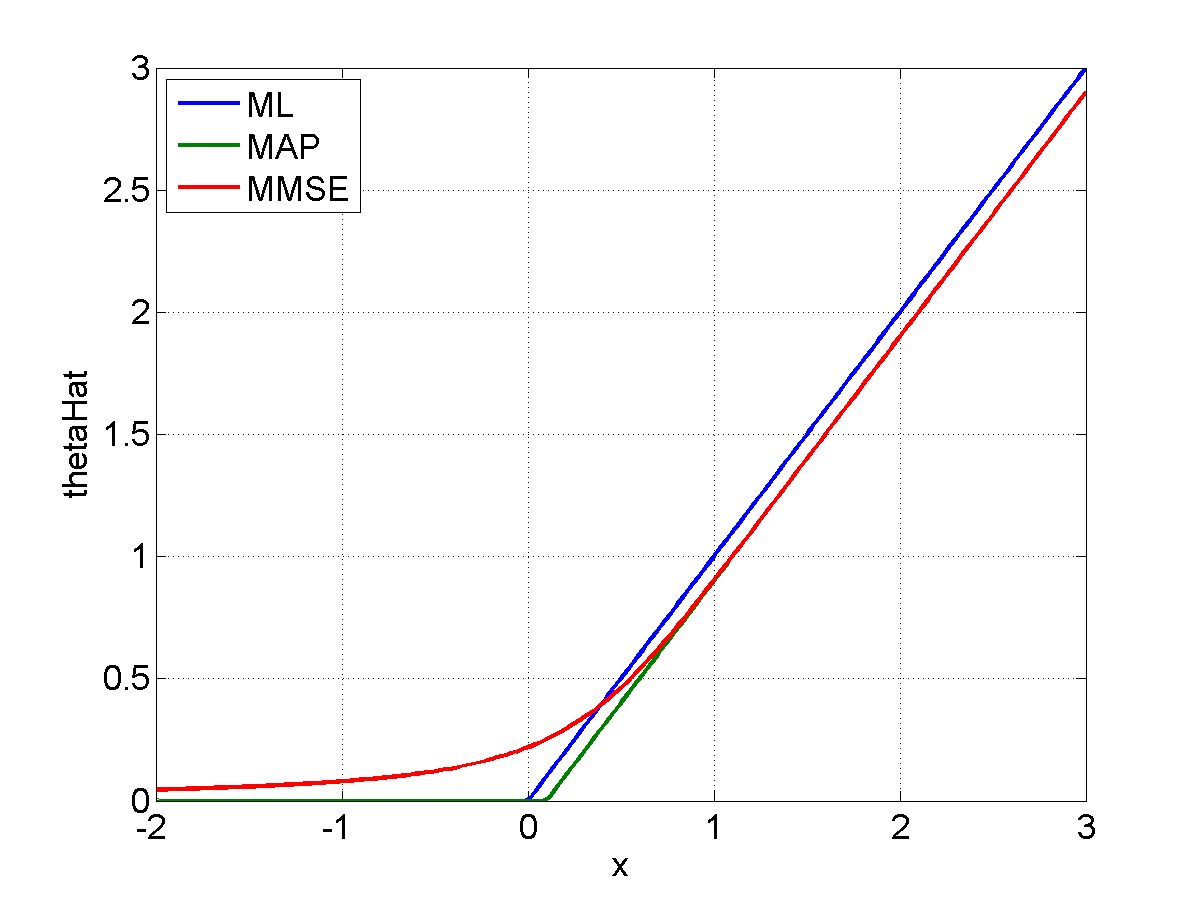
\includegraphics[width=.7\textwidth]{softThresh.png}
	\caption{Estimators for Problem \ref{prob:softThresh}.}
\label{fig:softThresh}
\end{figure}
\end{enumerate}

\item 
The expected loss is
\[
    J(\thetahat) = E(L(\theta,\thetahat)|x) = \int_{-\infty}^\infty |\theta-\thetahat|p(\theta|x)d\theta.
\]
We break this integral into two parts,
\[
    J(\thetahat) = \int_{\thetahat}^\infty (\theta-\thetahat)p(\theta|x)d\theta +
            \int_{-\infty}^\thetahat (\thetahat-\theta)p(\theta|x)d\theta.
\]
Using Leibnitz rule
\beqan
    \lefteqn{ \frac{\partial J(\thetahat)}{\partial \thetahat}
    = -(\thetahat-\thetahat)p(\thetahat|x) - \int_{\thetahat}^\infty p(\theta|x)d\theta
    +(\thetahat-\thetahat)p(\thetahat|x) + \int_{-\infty}^{\thetahat} p(\theta|x)d\theta }
    \\
    && = -P(\theta > \thetahat) + P(\theta \leq \thetahat).    \hspace{8cm}
\eeqan
Setting the derivative to zero, we obtain that
\[
    P(\theta > \thetahat) = P(\theta \leq \thetahat),
\]
which implies that $\thetahat$ is the median of the density, $p(\theta|x)$.

\item 

\begin{enumerate}[(a)]
\item The negative log likelihood is 
\[
    p(\xbf|\theta) = \prod_{i=1}^N p(x_i|\theta) = 
        \theta^N\prod_{i=1}^N e^{-\theta x_i},
\]
so the negative log likelihood is
\[
    L(\theta) = -\ln p(\xbf|\theta) = -N\ln(\theta)
        + \theta\sum_{i=1}^N x_i.
\]
Setting $L'(\theta) = 0$, we obtain
\[
    -\frac{N}{\theta} + \sum_{i=1}^N x_i \Rightarrow
    \thetahat = \left[ \frac{1}{N}\sum_{i=1}^N x_i\right]^{-1}.
\]

\item The Gamma distribution is
\[
    p(\theta) = \frac{\beta^\alpha}{\Gamma(\alpha)}
        \theta^{\alpha-1}e^{-\beta \theta} \propto \theta^{\alpha-1}e^{-\beta \theta},
\]
where the proportional to sign ($\propto$) indicates
a constant that does not depend on $\theta$.
Hence,
\[
    p(\theta|\xbf) \propto p(\xbf|\theta)p(\theta)
        \propto \theta^N\prod_{i=1}^N e^{-x_i\theta}
        \theta^{\alpha-1}e^{-\beta \theta}
        = \theta^{\alpha'-1}e^{-\beta' \theta},
\]
where
\[
    \alpha' = \alpha + N, \quad \beta' = \beta + \sum_{i=1}^N x_i.
\]

\item Let $\mu=\Exp(\theta)$, and $\tau = \var(\theta)$ be the prior
mean and variance.  We know from the wikipedia page on the Gamma
distribution,
\[
    \mu = \frac{\alpha}{\beta}, \quad \tau = \frac{\alpha}{\beta^2}
    \Rightarrow \beta = \frac{\mu}{\tau}, 
    \alpha = \frac{\mu^2}{\tau}.
\]
Hence, the posterior mean is
\[
    \Exp(\theta|\xbf) = \frac{\alpha'}{\beta'}
    = \frac{\alpha + N}{\beta + N\xbar}
    = \frac{\mu^2 + N\tau}{\mu + N\xbar \tau},
\]
where $\xbar = (1/N)\sum_i x_i$ is the sample mean.
The posterior variance is 
\[
    \var(\theta|\xbf) = \frac{\alpha'}{(\beta')^2}
    = \frac{\alpha + N}{(\beta + N\xbar)^2}
    = \tau \frac{\mu^2 + N\tau}{(\mu + N\xbar \tau)^2}.
\]

\item As $\tau \arr \infty$, 
\[
    \Exp(\theta|\xbf) \rightarrow \frac{1}{\xbar}, 
\]
which is the ML estimate.  This makes sense:  as $\tau \arr \infty$,
the prior becomes non-informative so the MMSE estimate converges to 
the MLE.

\end{enumerate}

\end{enumerate}

\end{document}

